\documentclass{article}
\usepackage{graphicx}
\usepackage{subfig}


\title{Problem Statement: Creating Provenance from System Call Traces}

\begin{document}
\maketitle

\begin{abstract}
This document gives a high level overview of the research project and its goals, as well as details on the inputs and expected end result.
\end{abstract}

\section{The research project}
Science is the art of coming up with questions and their answers, so it's always good to start with the questions. Obviously, there are lots of things we can do with the data, but here are a few things I'm trying to figure out.
\begin{enumerate}
\item Given a provenance graph, can we accurately predict what file people will access next?
\item In particular, can we figure out what ONE person will access next? (Personalized prediction)
\item Can we identify some characteristics of file access that are unique to bioinformatics?
\end{enumerate}

What we have right now is a bunch of long term system call traces from systems that have been used for computer science research, and a bioinformatics cluster that hasn't been installed yet. So we're focusing on turning the traces we have into a graph, and then once the cluster comes up, we can worry about getting traces from it. (Also, if we run into snags with the traces we have, we can avoid wasting time later)

\section{The data}
The data we're working with is from the LASR system.  It will look something like the following:
\begin{verbatim}
0 RESTART (scratch) at 962148771 Tue Jun 27 16:32:51 2000
28 RESTART (scratch) at 962583623 Sun Jul  2 17:20:23 2000
56 UID 0 PID 1 ?? A 962559820.187587 unlink("/etc/initrunlvl") = -1 (2)
96 UID 0 PID 1 ?? A 962559820.201366 unlink("/var/log/initrunlvl") = -1 (2)
140 UID 0 PID 10 ?? A 962559821.223185 unlink("/dev/log") = -1 (2)
176 UID 0 PID 10 ?? S 962559821.223242 exit(1280) = 0
\end{verbatim}

It's kind of obtuse, but you can see that there's a uid and a pid (user and process). There's a UNIX time stamp (like 962559821.223242), a system call name (like unlink), and then some arguments, and a return value.
\section{Provenance graphs}
A provenance graph has nodes, edges, and "annotations" (basically extra info). There are two kinds of nodes, processes and files. Edges connect files to processes, or vice versa, and are directed in order of data flow. So, for instance, if a process opens a file and reads it, then the edge goes from the file, to the process, because that's the direction the data went. For a write, the edge goes the other way, from the process to the file. If a process starts another process, we can think of that as data too (although it's a bit of a stretch), so the edge goes from the parent process to the child process. So here's some example graphs:

%USE SUBFIGURE
\begin{figure}[h!]
\subfloat[Process reads file][Process reads file]{
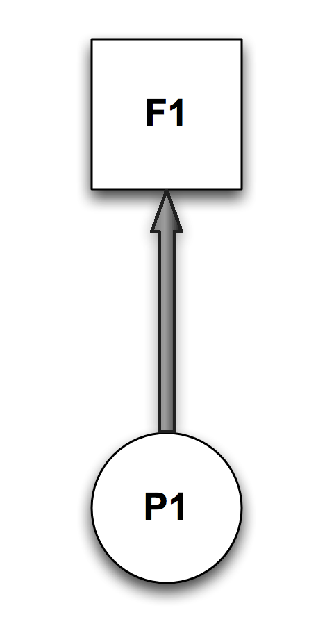
\includegraphics[width=0.4\textwidth]{figs/readfile}
\label{fig:subfig1}}


\subfloat[Process writes file][Process writes file]{
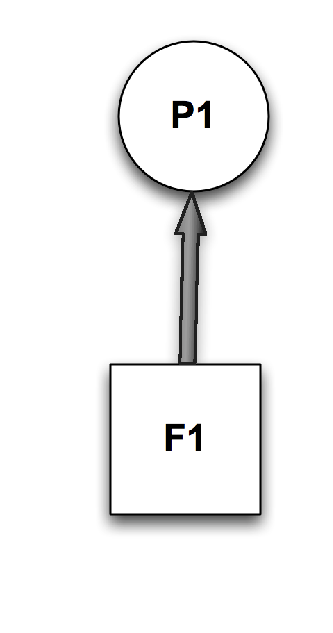
\includegraphics[width=0.4\textwidth]{figs/writefile}
\label{fig:subfig2}}


\subfloat[Process starts another process which reads one file, and then writes another.][Process starts another process which reads one file, and then writes another.]{
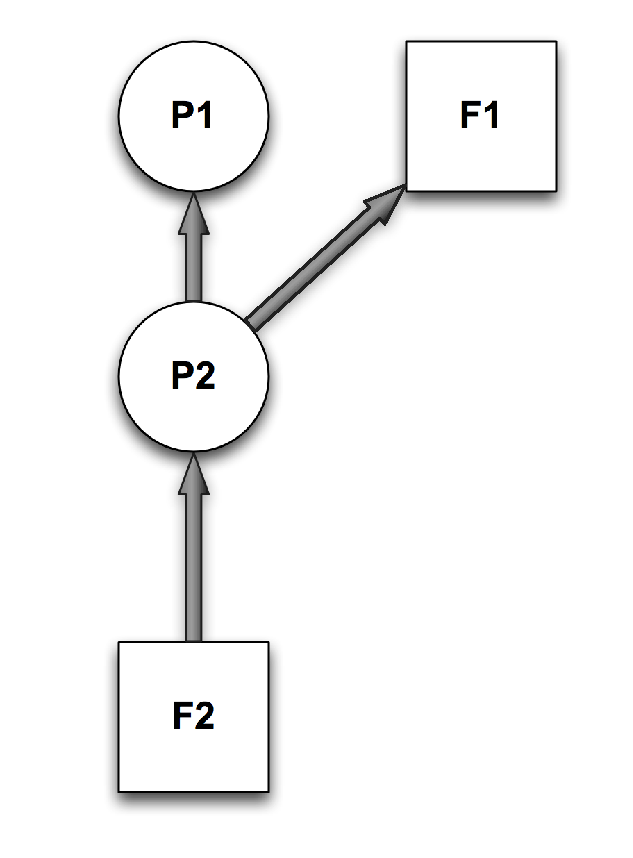
\includegraphics[width=0.4\textwidth]{figs/spawnreadwrite}
\label{fig:subfig3}}
\end{figure}

%\begin{figure}[h!]
%  \centering
%    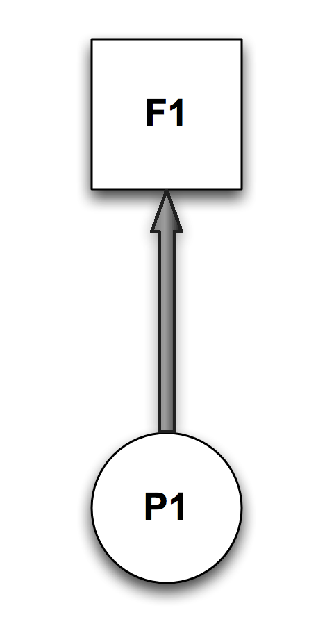
\includegraphics[width=.5\textwidth]{figs/readfile}
%      \caption{Process reads file.}
%      \label{fig:read}
%\end{figure}

%\begin{figure}[h!]
%  \centering
%    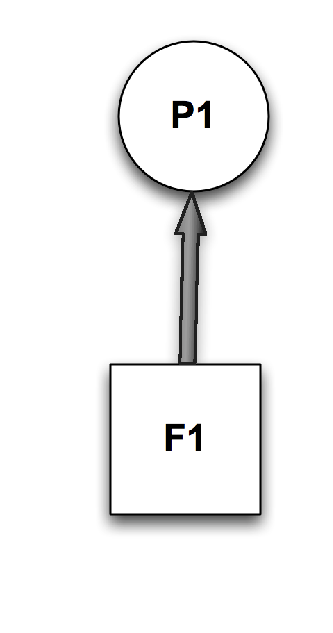
\includegraphics[width=.5\textwidth]{figs/writefile}
%      \caption{Process writes file.}
%      \label{fig:write}
%\end{figure}

%
%\begin{figure}[h!]
%  \centering
%    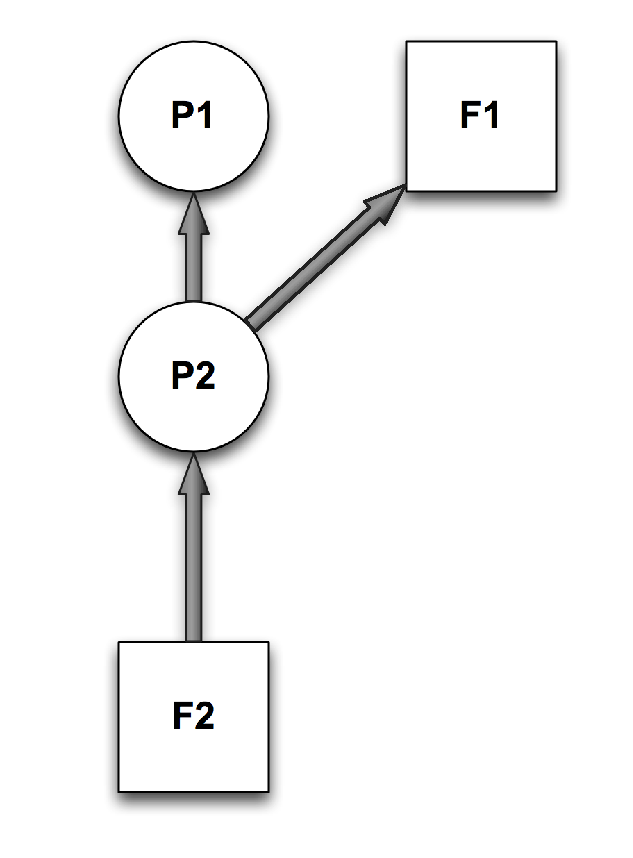
\includegraphics[width=.5\textwidth]{figs/spawnreadwrite}
%      \caption{Process starts another process which reads one file, and then writes another.}
%      \label{fig:spawnreadwrite}
%\end{figure}




However, that's not quite as much information as we need for full causality. So we add annotations, in the form of users, time stamps, and versions. When a file is changed, we declare that to be a new version of that file, so we might have results.txt(v1), results.txt(v2), etc. That way we can say which version of a file another file got data from, and we know which processes contributed up to that point.

Example graph:

\end{document}

